

\section{Quy trình Đề xuất và Theo dõi Lộ trình Học tập Cá nhân hóa}

\subsection{Tổng quan}
Hệ thống học tập trực tuyến thông minh được thiết kế để cung cấp trải nghiệm học tập cá nhân hóa, hỗ trợ học viên đạt được mục tiêu học tập một cách hiệu quả. Quy trình tận dụng trí tuệ nhân tạo (AI) để phân tích nhu cầu học viên, đề xuất nội dung phù hợp, đánh giá tiến độ, và điều chỉnh lộ trình học tập khi cần. Các chức năng chính bao gồm xây dựng lộ trình học tập, tạo bài kiểm tra tự động, theo dõi hiệu quả học tập, và tạo bổ sung nội dung để giải quyết khó khăn.

Quy trình được chia thành bốn giai đoạn chính:
\begin{itemize}
	\item Phân tích mục tiêu và tạo lộ trình học tập.
	\item Tạo bài kiểm tra tự động.
	\item Theo dõi và đánh giá tiến độ học tập.
	\item Điều chỉnh nội dung học tập dựa trên kết quả học tập.
\end{itemize}

\subsection{Giai đoạn 1: Phân tích Mục tiêu và Tạo Lộ trình Học tập}
Giai đoạn này tập trung vào việc hiểu mục tiêu học tập của học viên và xây dựng một kế hoạch học tập phù hợp, sử dụng AI để phân tích và đề xuất nội dung.
\begin{figure}[H]
    \centering
    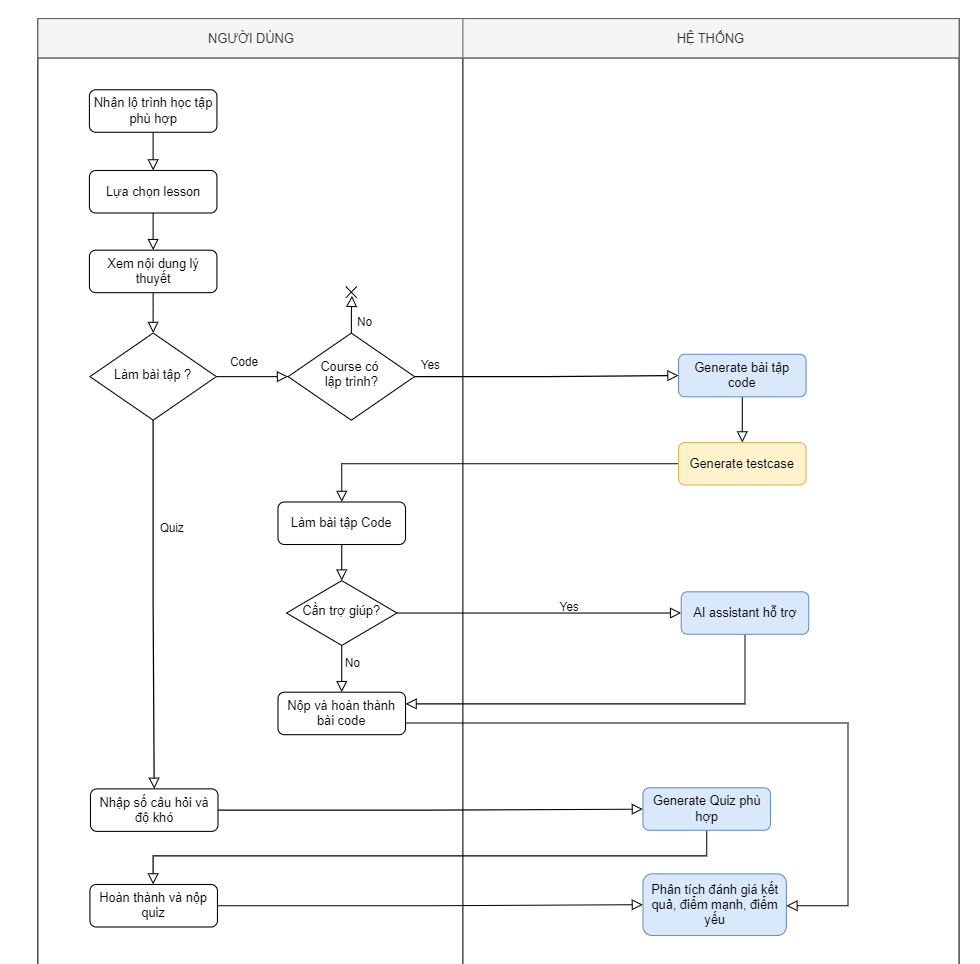
\includegraphics[width=\linewidth]{Images/flowchart_1.png}
    \caption{Giai đoạn 1: Phân tích Mục tiêu và Tạo Lộ trình Học tập}
\end{figure}
\begin{enumerate}
	\item \textbf{Hiểu mục tiêu học tập}: Hệ thống thu thập mục tiêu của học viên, ví dụ: ``nắm vững lập trình Python cơ bản'' hoặc ``cải thiện kỹ năng giải thuật''. AI phân tích mục tiêu để đảm bảo nó rõ ràng, phù hợp với khóa học, và khả thi trong thời gian quy định. Nếu mục tiêu có thời hạn cụ thể (như trước kỳ thi giữa kỳ), hệ thống xác định khoảng thời gian phù hợp.

	\item \textbf{Prompt sử dụng}:
	      \begin{Verbatim}[breaklines=true]
		      Phân tích mục tiêu học tập: "[goal]". Xác định tính hoàn chỉnh, phù hợp với khóa học "[course_name]", và khả thi dựa trên kết quả học tập mong đợi. Đề xuất dòng thời gian từ [start_date] đến [end_date]. Trả về JSON với start_date, end_date, và ghi chú xác thực.
	      \end{Verbatim}
	      Prompt này yêu cầu AI kiểm tra tính hợp lệ của mục tiêu và đề xuất thời gian thực hiện, đảm bảo lộ trình học tập phù hợp với lịch trình khóa học.

	\item \textbf{Lựa chọn bài học phù hợp}: AI xem xét nội dung khóa học và chọn các bài học liên quan nhất đến mục tiêu. Các bài học được sắp xếp từ cơ bản đến nâng cao, kèm theo giải thích về lý do lựa chọn, giúp học viên dễ dàng tiếp cận kiến thức.

	\item \textbf{Prompt sử dụng}:
	      \begin{Verbatim}[breaklines=true]
		      Dựa trên mục tiêu "[goal]" và khóa học "[course_name]", chọn các bài học từ danh sách [lessons_data]. Sắp xếp theo thứ tự logic, ưu tiên bài học cơ bản nếu thời gian ngắn. Trả về danh sách bài học với ID, thứ tự, tiêu đề, và lý do chọn.
	      \end{Verbatim}
	      Prompt này hướng dẫn AI lọc và sắp xếp bài học dựa trên mục tiêu, đảm bảo tính liên quan và trình tự hợp lý.

	\item \textbf{Xây dựng lộ trình chi tiết}: Hệ thống tạo lộ trình học tập bao gồm các bài học được chia thành các phần nhỏ (module), mỗi phần có nội dung lý thuyết, hướng dẫn thực hành, và tài liệu tham khảo. AI thiết kế lộ trình phù hợp với thời gian và tốc độ học của học viên.

	\item \textbf{Prompt sử dụng}:
	      \begin{Verbatim}[breaklines=true]
		      Tạo lộ trình học tập cho mục tiêu "[goal]" từ [start_date] đến [end_date]. Dựa trên bài học [selected_lessons], tạo danh sách bài học đề xuất với nội dung trọng tâm, giải thích lý do, và 2-3 module mỗi bài học. Trả về JSON với bài học và module chi tiết.
	      \end{Verbatim}
	      Prompt này yêu cầu AI tạo lộ trình chi tiết, bao gồm nội dung và module, để hỗ trợ học viên đạt mục tiêu một cách có hệ thống.
\end{enumerate}

\subsection{Giai đoạn 2: Tạo Bài Kiểm tra Tự động}
Hệ thống sử dụng AI để tạo bài kiểm tra nhằm đánh giá sự hiểu biết của học viên dựa trên nội dung học tập.
\begin{figure}[H]
    \centering
    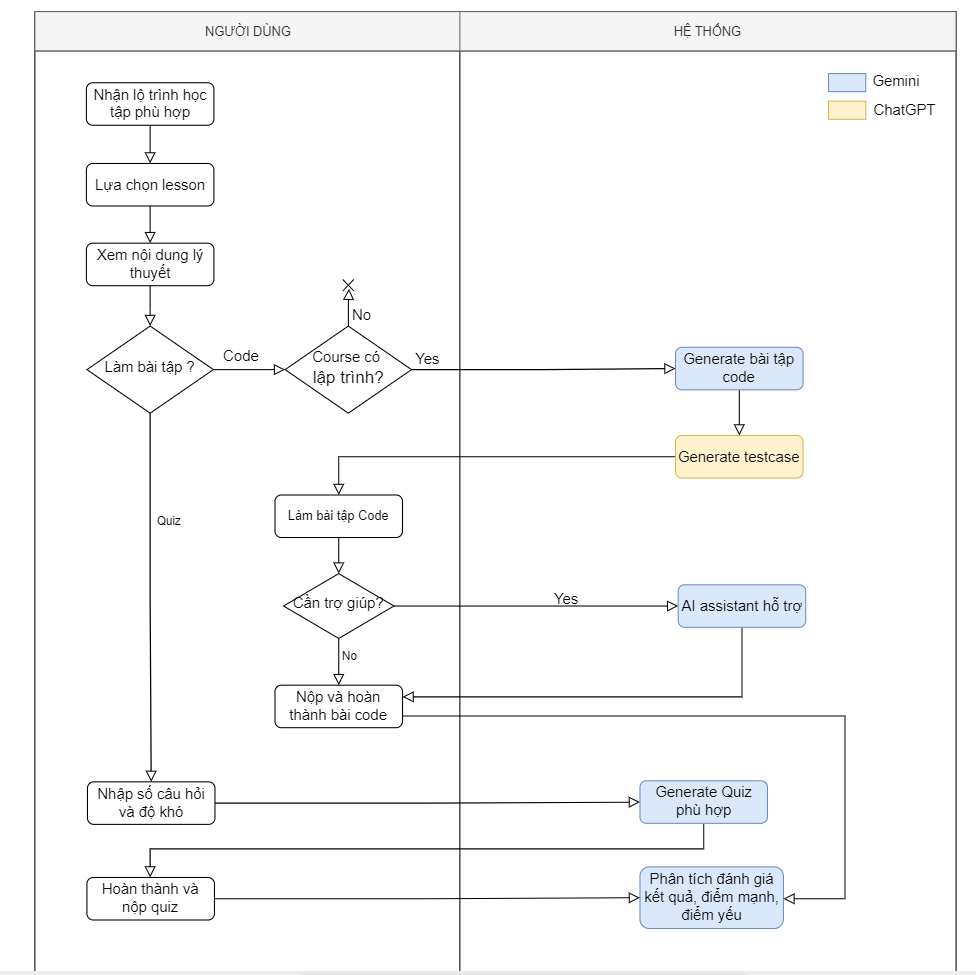
\includegraphics[width=\linewidth]{Images/flowchart_2.png}
    \caption{Giai đoạn 2: Học và làm bài kiểm tra}
\end{figure}
\begin{enumerate}
	\item \textbf{Xác định nội dung kiểm tra}: Hệ thống chọn một phần nội dung cụ thể (module) để tạo bài kiểm tra, tập trung vào các khái niệm và kỹ năng quan trọng.

	\item \textbf{Tạo câu hỏi đa dạng}: AI tạo các câu hỏi với nhiều mức độ khó (dễ, trung bình, khó) và loại hình (trắc nghiệm đơn, đa lựa chọn, đúng/sai). Mỗi câu hỏi đi kèm giải thích chi tiết để học viên hiểu rõ đáp án.

	\item \textbf{Prompt sử dụng}:
	      \begin{Verbatim}[breaklines=true]
		      Tạo [count] câu hỏi [difficulty] cho module "[module_title]". Câu hỏi dựa trên mục tiêu [objectives] và nội dung "[recommended_content]". Bao gồm loại câu hỏi đa dạng (single_choice, multiple_choice, true_false), với giải thích chi tiết. Trả về JSON với câu hỏi, lựa chọn, đáp án, và điểm.
	      \end{Verbatim}
	      Prompt này chỉ đạo AI tạo câu hỏi phù hợp với nội dung module, đảm bảo đa dạng và có giá trị đánh giá cao.

	\item \textbf{Thiết lập thông tin bài kiểm tra}: Hệ thống đặt thời gian làm bài và tổng điểm dựa trên số lượng câu hỏi, đảm bảo bài kiểm tra cân đối và khả thi.

	\item \textbf{Prompt sử dụng}:
	      \begin{Verbatim}[breaklines=true]
		      Thiết lập bài kiểm tra cho module "[module_title]". Dựa trên [questions_count] câu hỏi, tính thời gian làm bài (2 phút/câu, tối đa 60 phút) và tổng điểm. Trả về JSON với tên, mô tả, thời gian, và điểm tối đa.
	      \end{Verbatim}
	      Prompt này giúp AI cấu hình bài kiểm tra phù hợp với khối lượng nội dung, đảm bảo trải nghiệm học tập công bằng.
\end{enumerate}

\subsection{Giai đoạn 3: Theo dõi và Đánh giá Tiến độ Học tập}
Hệ thống liên tục theo dõi quá trình học tập của học viên, sử dụng AI để đánh giá và đưa ra gợi ý cải thiện.
\begin{figure}[H]
    \centering
    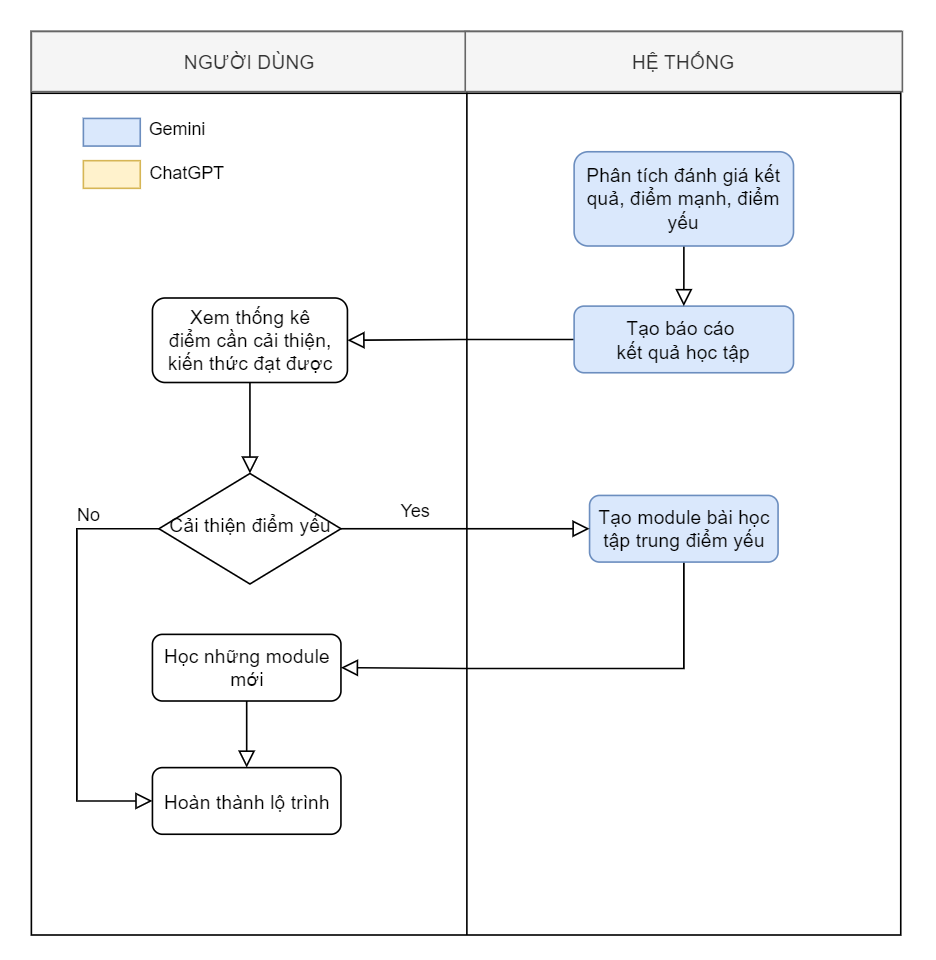
\includegraphics[width=\linewidth]{Images/flowchart_3.png}
    \caption{Giai đoạn 3: Theo dõi và Đánh giá Tiến độ Học tập}
\end{figure}
\begin{enumerate}
	\item \textbf{Thu thập dữ liệu học tập}: Hệ thống ghi nhận thời gian học, tiến độ hoàn thành bài học, và kết quả bài kiểm tra, từ đó đánh giá mức độ nỗ lực và hiểu biết của học viên.

	\item \textbf{Đánh giá theo tiêu chí}: AI phân tích tiến độ dựa trên ba yếu tố:
	      \begin{itemize}
		      \item \textit{Kiến thức lý thuyết}: Mức độ hiểu các khái niệm quan trọng.
		      \item \textit{Kỹ năng thực hành}: Khả năng áp dụng kiến thức, như viết mã lập trình.
		      \item \textit{Mức độ nỗ lực}: Sự chăm chỉ, dựa trên thời gian học và số bài học đã bắt đầu.
	      \end{itemize}

	\item \textbf{Prompt sử dụng}:
	      \begin{Verbatim}[breaklines=true]
		      Đánh giá tiến độ học viên "[student_name]" với mục tiêu "[goal]". Dựa trên dữ liệu bài học [lessons_data], phân tích theo kiến thức lý thuyết, kỹ năng thực hành, và nỗ lực. Trả về JSON với báo cáo STAR, điểm mạnh, điểm cần cải thiện, và gợi ý chi tiết.
	      \end{Verbatim}
	      Prompt này yêu cầu AI tạo báo cáo toàn diện, giúp học viên hiểu rõ tình trạng học tập và nhận gợi ý cụ thể.

	\item \textbf{Báo cáo chi tiết}: AI tạo báo cáo nêu rõ điểm mạnh (như nắm vững lý thuyết), điểm cần cải thiện (như kỹ năng thực hành còn yếu), và gợi ý (như tập trung vào bài tập thực hành). Báo cáo được trình bày rõ ràng để học viên dễ áp dụng.
\end{enumerate}

\subsection{Giai đoạn 4: Điều chỉnh Nội dung Học tập}
Khi học viên gặp khó khăn, hệ thống sử dụng AI để phân tích và tái tạo nội dung học tập, giúp giải quyết vấn đề hiệu quả.

\begin{enumerate}
	\item \textbf{Phân tích vấn đề}: AI xem xét các khó khăn, như hiểu sai khái niệm hoặc mắc lỗi thực hành, và xác định liệu học viên cần ôn lại nội dung trước đó.

	\item \textbf{Prompt sử dụng}:
	      \begin{Verbatim}[breaklines=true]
		      Phân tích vấn đề từ dữ liệu [issues_summary] cho bài học "[lesson_title]". Xác định các khó khăn chính (hiểu sai, lỗi thực hành) và đề xuất hành động (lặp lại, xem lại bài trước). Trả về JSON với danh sách vấn đề, mức độ nghiêm trọng, và hành động đề xuất.
	      \end{Verbatim}
	      Prompt này giúp AI xác định nguyên nhân khó khăn và đề xuất cách khắc phục phù hợp.

	\item \textbf{Tái tạo nội dung}: AI tạo lại nội dung bài học, tập trung vào giải quyết các vấn đề đã xác định. Nội dung mới bao gồm ví dụ thực tế, hướng dẫn chi tiết, và tài liệu tham khảo phù hợp.

	\item \textbf{Prompt sử dụng}:
	      \begin{Verbatim}[breaklines=true]
		      Tái tạo nội dung cho bài học "[lesson_title]" dựa trên vấn đề [issues_analysis]. Cung cấp nội dung mới với giải thích chi tiết, ví dụ thực tế, và 2-3 module tập trung vào khó khăn. Trả về JSON với nội dung đề xuất, giải thích, và module.
	      \end{Verbatim}
	      Prompt này chỉ đạo AI thiết kế nội dung mới, đảm bảo phù hợp với nhu cầu cụ thể của học viên.

	\item \textbf{Cập nhật lộ trình}: Nội dung mới được tích hợp vào lộ trình học tập, giúp học viên tiếp tục học mà không bị gián đoạn.
\end{enumerate}

\subsection{Kết luận}
Quy trình đề xuất và theo dõi lộ trình học tập cá nhân hóa tận dụng trí tuệ nhân tạo để mang lại trải nghiệm học tập linh hoạt và hiệu quả. Các câu lệnh AI (prompt) được thiết kế cẩn thận để phân tích mục tiêu, tạo nội dung, đánh giá tiến độ, và điều chỉnh lộ trình, giúp học viên vượt qua khó khăn và đạt được mục tiêu học tập. Quy trình này không chỉ nâng cao chất lượng học tập mà còn đảm bảo sự hỗ trợ liên tục, phù hợp với từng cá nhân.
